\documentclass[a4paper,10pt]{article}
\usepackage[utf8]{inputenc}
\usepackage{dsfont, graphicx}

%opening
\title{Incomplete quantum tomography using neural networks}
\author{Olivia Di Matteo}

\begin{document}

\maketitle

\section{Problem formalism}

The goal of quantum tomography is, given (many identical copies of) some arbitrary quantum state, take a series of measurements in order to determine its density matrix. When the dimension of the system $d$ is prime ($p$), or power of prime ($p^n$), a complete set of $d + 1$ bases that are mutually unbiased comprise an optimal set of measurements. These can be written in vector form, but another common way of expressing them is as $d + 1$ sets of $d - 1$ commuting observables (total of $d^2-1$) which have as mutual eigenvectors bases that are MU.

A density matrix $\rho$ can be expressed in terms of $d^2 - 1$ parameters; while an arbitrary complex $d \times d$ matrix contains $2d^2$ entries, the hermiticity and the condition on the trace of a density matrix, i.e. $\hbox{Tr}(\rho) = 1$ reduce the number of parameters required. A convenient way, for our purposes, is expressing the density matrix in terms of its expansion coefficients in an operator basis:
\begin{equation}
 \rho = \frac{1}{d} \mathds{1} + \frac{1}{d} \sum_{i = 1}^{d^2 - 1} a_i P_i
\end{equation}
\noindent For example, we might choose the Pauli basis, and then this expression is the $d$-dimensional analogue of the 2-dimensional Bloch vector.

The goal of a tomographic process would then be, given some measurement data, to estimate the values of the coefficients $a_i$.

\section{Basic version: Incomplete tomography using neural networks}

If we consider multi-qubit systems, i.e. $d = 2^n$, the number of measurements required scales poorly with the number of qubits. As larger numbers of qubits become experimentally tractable, we will need effective methods of incomplete tomography to make the reconstruction process feasible. Efforts in this direction have involved compressed sensing, and least-bias maximum-likelihood state estimation (LBMLE). We propose here a method based on neural networks. The idea here is that the networks can be trained to reconstruct states based on simulated incomplete experimental data; this allows the heavy lifting to be done computationally, as one needs only train the network once, and then feed it the ``real'' experimental results. There is also a huge amount of versatility as one can very simply adapt the process to train using whatever measurements are taken in a particular experimental setup.

We propose a very simple feed-forward neural network for this task. 
The network in question is shown in figure \ref{fig:nn}. The input layer consists of the measurement frequencies. These are generated `experimentally' by computing the set of projectors for each of the chosen measurement bases, and the probability of that outcome via the Born rule. Then we use MC simulation to generate frequencies of each outcome. The output layer consists of the basis coefficients above, the $a_i$.

\begin{figure}
 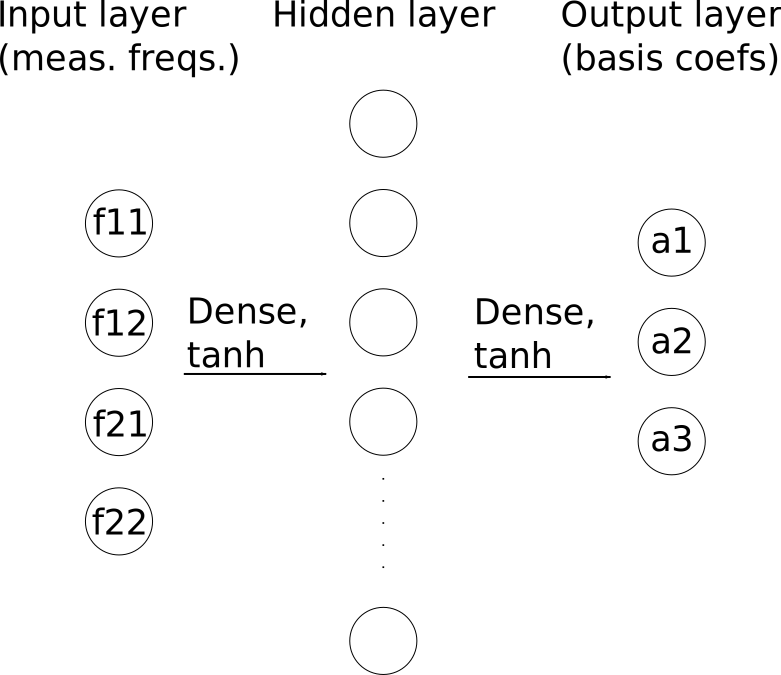
\includegraphics[scale=0.5]{nn_schematic}
 \caption{Simple diagram of neural network. The measurement frequencies from each measured basis are passed in as input nodes. The hidden layer seems to work well with a quadratic number of nodes, after which there are diminishing returns. The output layer should have $d^2 - 1$ nodes.}
 \label{fig:nn}
\end{figure}


In theory this should work great; in practice we need to determine the properties of the hidden layer that are the most effective for this purpose. First, the activation functions. The output vector of coefficients must be normalized, and can contain both positive and negative quantities. We therefore choose tanh as the activation function, as it takes a range (-1, 1). We then manually normalize the output vector so that it is a pure quantum state. For a loss function, we choose the cosine proximity. In essence, this serves to measure the angle between the true and predicted (normalized) vectors; physically, for a single qubit, this would correspond to the angle between vectors on the Bloch sphere, which seems like a sensible thing to try and minimize.


As proof of concept, we have trained the network to reconstruct a single qubit pure state. We trained our network with 9000 Haar-random pure states, and tested on 1000 additional ones. As a metric of success, we choose the fidelity. 

Training the network with all 3 MUBs yields an average fidelity of 0.9999, which is a solid sanity check. We then attempt to train it using simulated measurement data from only 2 of the 3 MUBs.  Our network reconstructs states with a fidelity of 0.944 on average; this can be compared, using the same test data, with the LBMLE algorithm, which reconstructs the states with an average of 0.91.

The distribution of the output fidelities is shown in figure \ref{fig:fids_dim2}. We see that the output of the neural network is more peaked at higher fidelities, whereas that of the LBMLE is more broad.
\begin{figure}
 \includegraphics[scale=0.5]{fids_dim2}
 \caption{Density of the output fidelities for reconstruction using neural network vs. LBMLE algorithm. The bases used were the eigenvectors of Pauli $X$ and $Z$.}
 \label{fig:fids_dim2}
\end{figure}

\section{Angular dependence of reconstructions}

One important thing to consider is the quality of the data set that goes into the network training. We used Haar-random states (HRS), which are generated by hitting a fiducial state by a Haar-random unitary (HRU). HRUs are distributed in a distinct way; in particular, the "weight" factor in the measure of integration is 
\begin{equation} 
 dU \simeq \sin \beta d\alpha d\beta d\gamma
\end{equation}
where $\alpha, \beta, \gamma$ are the 3 parameters which allow us to construct the matrix
\begin{equation}
 U(\alpha, \beta, \gamma) = \left( 
  \begin{array}{cc}
   e^{i \alpha} \cos( \beta/2) & -e^{i \gamma} \sin(\beta / 2) \\
    e^{-i \gamma} \sin(\beta / 2) & e^{-i \alpha} \cos( \beta/2) 
  \end{array}
  \right)
\end{equation}
 (more technically this is SU(2) rather than U(2) I guess). This looks very similar to the integration measure in spherical coordinates, when integrating over a sphere of radius 1. In this sense, $\beta$ plays the role of the polar angle $\theta$. The extra factor of $\sin \beta$ adds takes its maximum value at $\beta = \pi / 2$, namely at the equator of the sphere; there is consequently more `weight' added to these states, meaning that equatorial states are more likely to occur than, say, polar states, when randomly sampling from the distribution of HRUs.
 
 To that end, I was initially concerned that using a training dataset based on HRS would mean that there are more states around the equator, and that consequently we would be able to learn these states better than the polar states. So I decided to plot the polar angle of the states on the Bloch sphere vs the fidelity of the reconstruction from the two different methods. I did this for all 3 combinations of measurement bases, ZY, XY, and ZX. Results for ZY and ZX were practically identical; the main differences lie between e.g. ZY and XY.
 
 \begin{figure}
  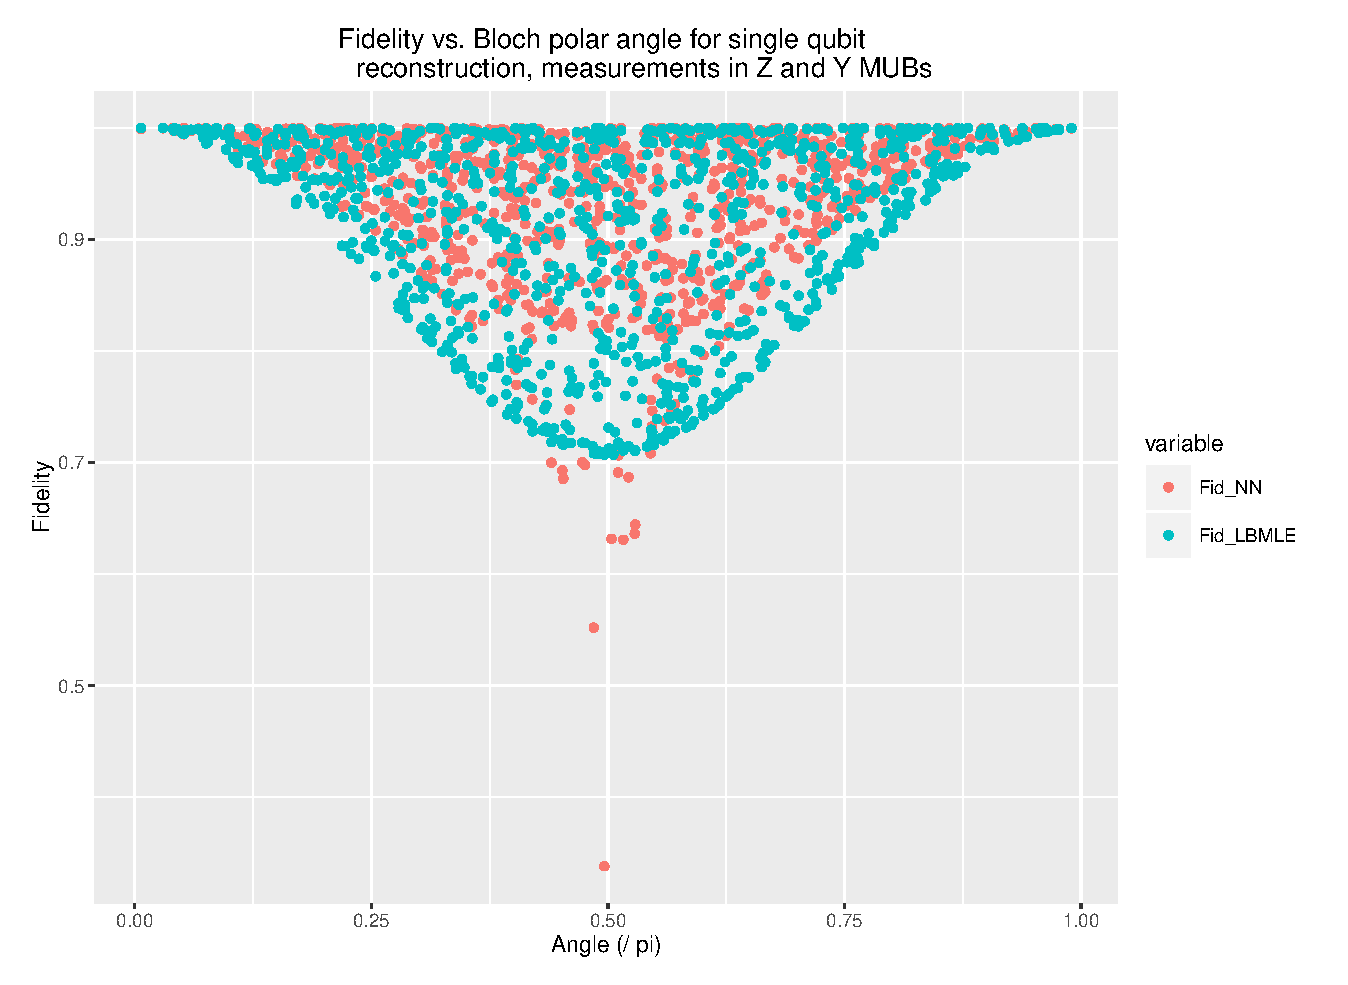
\includegraphics[scale=0.6]{fid_v_angle_zy}
  \caption{Fidelity of reconstruction vs angle with measurement data from the Z and Y MUBs.}
  \label{fig:fid_v_angle_zy}
 \end{figure}
 
  \begin{figure}
  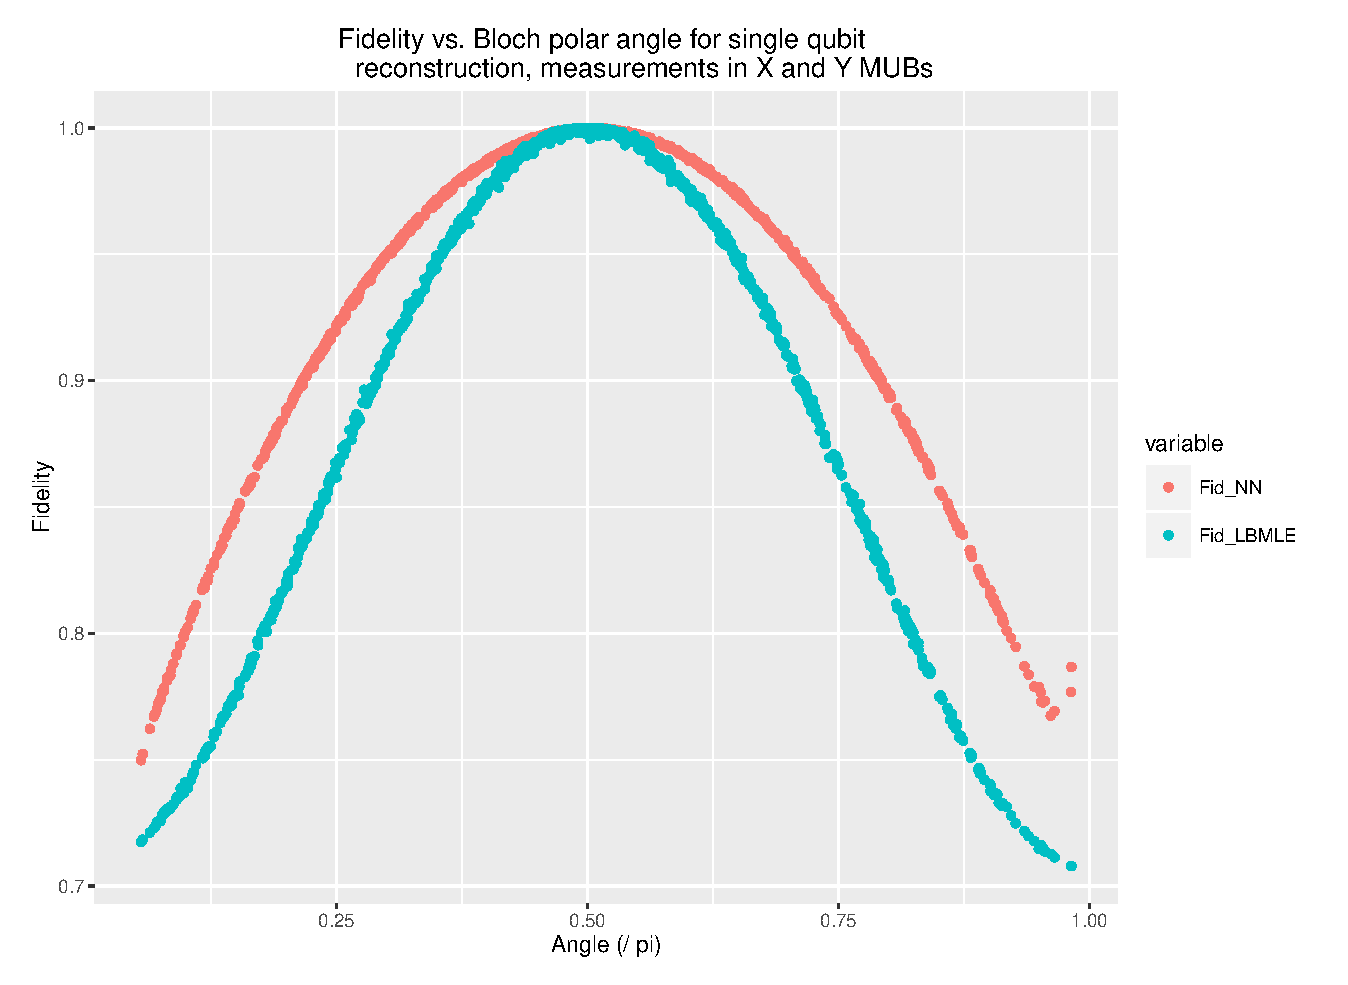
\includegraphics[scale=0.6]{fid_v_angle_xy}
  \caption{Fidelity of reconstruction vs angle with measurement data from the X and Y MUBs.}
  \label{fig:fid_v_angle_xy}
 \end{figure}
 
 The first thing to note is that it doesn't seem that the distribution of the data set has much effect; I make this conclusion because when we reconstruct with the ZY bases, the states in the middle (i.e. angle ~ $\pi/2$) are more poorly reconstructed than the polar states, despite there being more of them in the training set. What \emph{does} make a huge difference is the bases we choose to measure in.
 
 The X and Y axes are those defining the equator of the Bloch sphere, and so it makes sense that measuring in those basis will give us better reconstructions simply because there is more `room to move around' in this portion of the sphere. There is, in a sense, more room for error here and so we want to learn as much as we can about how things related to these two axes vs. the polar one. 
 
 What's more interesting though is the differences between the two algorithms. The average fidelity for the neural network is pretty much the same whether we use ZY or XY. However for both algorithms, the fidelity for the XY case is far more correlated with angle. The LBMLE looks normally distributed in both cases but for the ZY measurements the normal distribution is filled in, while for XY the points simply follow the outline of a bell curve. 
 
 For the ZY case, the neural network looks like it fares worse closer to the middle (which I feel makes sense as we are using the cosine proximity as a loss function). However the average is still superior because the fidelity of the polar states is handled better than in LBMLE. In the XY case again the NN handles the polar states better, and it looks more paraboloid than it does normal. \\
 
 Some obvious questions to consider next:
 \begin{itemize}
  \item What happens for mixed states? Does the neural network still fare well? We cannot normalize it now, it may live inside the Bloch sphere. How do we ensure that the output is always a vector < 1?
  \item Can we generalize these ideas to higher dimensions? e.g. in dimension 4, can we pick bases that span the most probable parts of the space in the same way that we X and Y span the equatorial region in the case of a single qubit?
 \end{itemize}
 
\end{document}
